\subsection{QLoRA Adaptation with Three Training Seeds}
\label{sec:qlora_results}
Nine adapter fits completed all twelve preserved tests, giving 216,000
paired base/adapted predictions and 1,800 serial benchmark predictions.
Each fit is evaluated separately on the same 3,000 records per condition;
Table~\ref{tab:qlora_paired} and Fig.~\ref{fig:qlora_paired} report
means and sample standard deviations over three training seeds.
Balanced mean weighted-F1 gains range from 3.21 to 9.72 percentage
points. Adapted means lie between 0.7833 and 0.7857; these nearby point
estimates do not establish model-to-model superiority.
% Generated by export_qlora_manuscript.py from verified saved predictions.
\begin{table}[tb]
\centering
\footnotesize
\setlength{\tabcolsep}{3pt}
\caption{Paired HF base/QLoRA weighted F1 on 500-character tests. Each mode uses 3,000 pooled records; all adapters use 500 training and 2,000 validation records. A: balanced; B: reduced imbalance. Gains and paired 95\,\% intervals are in percentage points.}
\label{tab:qlora_paired}
\begin{tabular}{llrrrr}
\toprule
Model & Condition & Base F1 & QLoRA F1 & $\Delta$ (pp) & 95\,\% CI ($\Delta$) \\
\midrule
Gemma 4 & A & 0.7520 & 0.7803 & +2.83 & [1.75, 3.96] \\
Gemma 4 & B & 0.7730 & 0.7948 & +2.18 & [1.12, 3.22] \\
Qwen3 & A & 0.7099 & 0.7891 & +7.92 & [6.55, 9.34] \\
Qwen3 & B & 0.7278 & 0.7946 & +6.68 & [5.30, 8.07] \\
Phi-4 & A & 0.6883 & 0.7845 & +9.62 & [8.21, 11.07] \\
Phi-4 & B & 0.7456 & 0.7994 & +5.38 & [4.08, 6.68] \\
\bottomrule
\end{tabular}
\end{table}
\begin{table}[tb]
\centering
\footnotesize
\setlength{\tabcolsep}{3pt}
\caption{Local resource measurements for 500-training-record adapters. Latency: warm batch-1 mean on the same 100 balanced 500-character records per mode, including prompt preparation and generation. Training time includes validation/checkpointing and excludes initial weight loading. Memory is peak allocated CUDA memory, not total GPU utilisation.}
\label{tab:qlora_resources}
\begin{tabular}{lrrrr}
\toprule
Model & Base (s) & QLoRA (s) & Train (min) & Peak (GiB) \\
\midrule
Gemma 4 & 0.475 & 0.647 & 34.75 & 7.77 \\
Qwen3 & 0.421 & 0.539 & 41.15 & 10.04 \\
Phi-4 & 0.487 & 0.435 & 40.68 & 9.32 \\
\bottomrule
\end{tabular}
\end{table}


Within this paired test design's 36 model--training-seed--condition--length comparisons,
34 unadjusted 95\,\% paired F1-change intervals exclude zero in the positive direction.
34 accuracy comparisons pass Holm correction across this family
of 36 tests. These within-fit intervals measure uncertainty conditional
on saved test outputs; between-fit variation is reported separately.
The two intervals containing zero are Gemma seed 2 under reduced
imbalance at both character limits; their point gains remain positive,
but a reliable improvement is not established in those two comparisons.
Overlapping conditions and narrative variants are not independent replications.
There are 4 invalid adapted predictions among 108,000 outputs,
compared with 73 invalid base outputs. Invalid responses remain errors.
Supplementary Table~\ref{S-tab:replication_full} reports every fit and condition.

\begin{figure}[tb]\centering
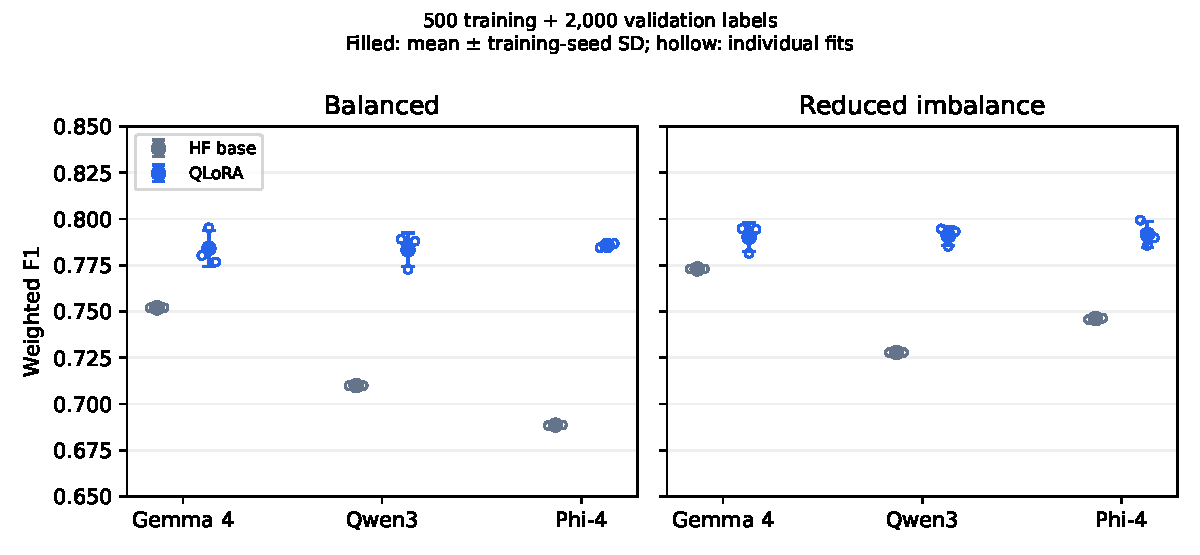
\includegraphics[width=\textwidth]{figures/v2/hf_qlora_multiseed_f1.pdf}
\caption{Matched HF base/adapted mean weighted F1 over three training
seeds on identical 3,000-record tests. Error bars show sample standard
deviation over fits, not bootstrap confidence intervals. Hollow points
show individual fits; the displayed vertical range is 0.65--0.85.}
\label{fig:qlora_paired}\end{figure}

The label-matched classifier comparison uses the same 500 training and
2,000 validation records. The validation-stopped DistilBERT control
has balanced weighted F1 0.7150
$\pm$ 0.0208; the fixed
three-epoch control scores 0.5329
$\pm$ 0.1522.
TF-IDF/SVM scores 0.7546 at the same training-label budget.

Per-fit adapter--classifier F1 differences use paired cluster bootstrap;
accuracy tests correct a separate family of 72 comparisons covering
three models, three fit seeds, two conditions, two lengths and two classifiers.
On balanced 500-character tests, all nine adapter--SVM F1-change
intervals are positive. The corresponding Holm-adjusted accuracy tests
pass for all three Phi fits and two fits each for Gemma and Qwen;
the remaining Gemma/Qwen comparisons have adjusted $p$ values
0.0768 and 0.0812. All nine comparisons with validation-stopped
DistilBERT pass the adjusted accuracy test. These accuracy tests and
unadjusted F1 intervals address different estimands and multiplicity.
The complete differences and adjusted tests are supplied as reproducibility CSVs;
no model-to-model superiority is inferred from point estimates alone.

Supplementary Table~\ref{S-tab:replication_class} reports class F1
over all three fits. Under reduced imbalance, mean adapted credit-card
F1 ranges from 0.6398 to 0.6660 while credit-reporting F1 ranges
from 0.8481 to 0.8511. Thus the high weighted scores do not remove
minority-class weaknesses, including after adaptation.

Table~\ref{tab:qlora_resources} reports training and serial timing.
Adapted balanced serial means range from 0.436 to
0.656~s across model averages. These measurements concern
unmerged adapters and a fixed 100-record warm serial benchmark per fit,
not concurrent throughput. The same benchmark records a decrease in
Phi-4's mean output length from 13.01 tokens without its adapter to
9.34 with it; Gemma and Qwen remain near 9.5 and 9.3 tokens in both
modes. Shorter Phi completions are consistent with its latency reduction,
but output length and adapter execution are not independently manipulated,
so their timing contributions cannot be isolated from these measurements.
Supplementary Section~\ref{S-sec:serial_tokens} reports the per-fit counts.
Full-test F1 uses batched outputs; verification scripts compare source
hashes, labels, saved responses and artifacts and record serial/batch
prediction differences separately.
